\let\negmedspace\undefined
\let\negthickspace\undefined
\documentclass[journal]{IEEEtran}
\usepackage[a5paper, margin=10mm, onecolumn]{geometry}
\usepackage{tfrupee} 

\setlength{\headheight}{1cm} 
\setlength{\headsep}{0mm}     

\usepackage{gvv-book}
\usepackage{gvv}
\usepackage{cite}
\usepackage{amsmath,amssymb,amsfonts,amsthm}
\usepackage{algorithmic}
\usepackage{graphicx}
\usepackage{textcomp}
\usepackage{xcolor}
\usepackage{txfonts}
\usepackage{listings}
\usepackage{enumitem}
\usepackage{mathtools}
\usepackage{gensymb}
\usepackage{comment}
\usepackage[breaklinks=true]{hyperref}
\usepackage{tkz-euclide} 
\usepackage[latin1]{inputenc}                                
\usepackage{color}                                            
\usepackage{array}                                            
\usepackage{longtable}                                       
\usepackage{calc}                                             
\usepackage{multirow}                                         
\usepackage{hhline}                                           
\usepackage{ifthen}                                           
\usepackage{lscape}

\begin{document}

\bibliographystyle{IEEEtran}
\vspace{3cm}

\title{2.9.24}
\author{AI25BTECH11008 - Chiruvella Harshith Sharan}
{\let\newpage\relax\maketitle}

% Ensure sequential numbering
\renewcommand{\theequation}{\arabic{equation}}
\renewcommand{\thefigure}{\arabic{figure}}
\renewcommand{\thetable}{\arabic{table}}

\setlength{\intextsep}{10pt} 

\textbf{Question}: 2.9.24 Find the co-ordinates of the point where the line
\[
\vec{r} = (-\hat{i}-2\hat{j}-3\hat{k}) + \lambda(3\hat{i}+4\hat{j}+3\hat{k})
\]
meets the plane which is perpendicular to the vector
\[
\vec{n} = \hat{i} + \hat{j} + 3\hat{k}
\]
and at a distance of $\frac{4}{\sqrt{11}}$ from origin.\\\\


\textbf{Solution}: \\\\[0.3cm]

The parametric form of the line is
\begin{equation}
\vec{r}(\lambda) = \myvec{-1 \\ -2 \\ -3} + \lambda\myvec{3 \\ 4 \\ 3}
= \myvec{-1+3\lambda \\ -2+4\lambda \\ -3+3\lambda}.
\end{equation}

The equation of the plane with normal $\vec{n}$ and distance $d=\tfrac{4}{\sqrt{11}}$ from origin is
\begin{equation}
\vec{n}^T\vec{r} = \pm \|\vec{n}\| d.
\end{equation}

Now,
\begin{equation}
\|\vec{n}\| = \sqrt{1^2 + 1^2 + 3^2} = \sqrt{11},
\quad
\pm \|\vec{n}\| d = \pm 4.
\end{equation}

So the plane equations are
\begin{equation}
\vec{n}^T \vec{r} = 4
\quad \text{or} \quad
\vec{n}^T \vec{r} = -4.
\end{equation}

Substitute $\vec{r}(\lambda)$:
\begin{equation}
\vec{n}^T \vec{r}(\lambda) = (1)(-1+3\lambda) + (1)(-2+4\lambda) + (3)(-3+3\lambda).
\end{equation}

Simplifying,
\begin{equation}
\vec{n}^T \vec{r}(\lambda) = -1+3\lambda -2+4\lambda -9+9\lambda
= -12 + 16\lambda.
\end{equation}

Case 1: 
\begin{equation}
-12 + 16\lambda = 4 \quad \Rightarrow \quad \lambda = 1.
\end{equation}

Case 2:
\begin{equation}
-12 + 16\lambda = -4 \quad \Rightarrow \quad \lambda = \tfrac{1}{2}.
\end{equation}

Hence, the intersection points are:
\begin{equation}
\vec{r}(1) = \myvec{2 \\ 2 \\ 0},
\quad
\vec{r}\left(\tfrac{1}{2}\right) = \myvec{\tfrac{1}{2} \\ 0 \\ -\tfrac{3}{2}}.
\end{equation}

\textbf{Final Answer}: The required points are
\begin{equation}
(2,2,0) \quad \text{and} \quad \left(\tfrac{1}{2},0,-\tfrac{3}{2}\right).
\end{equation}

\begin{figure}[htbp]
    \centering
    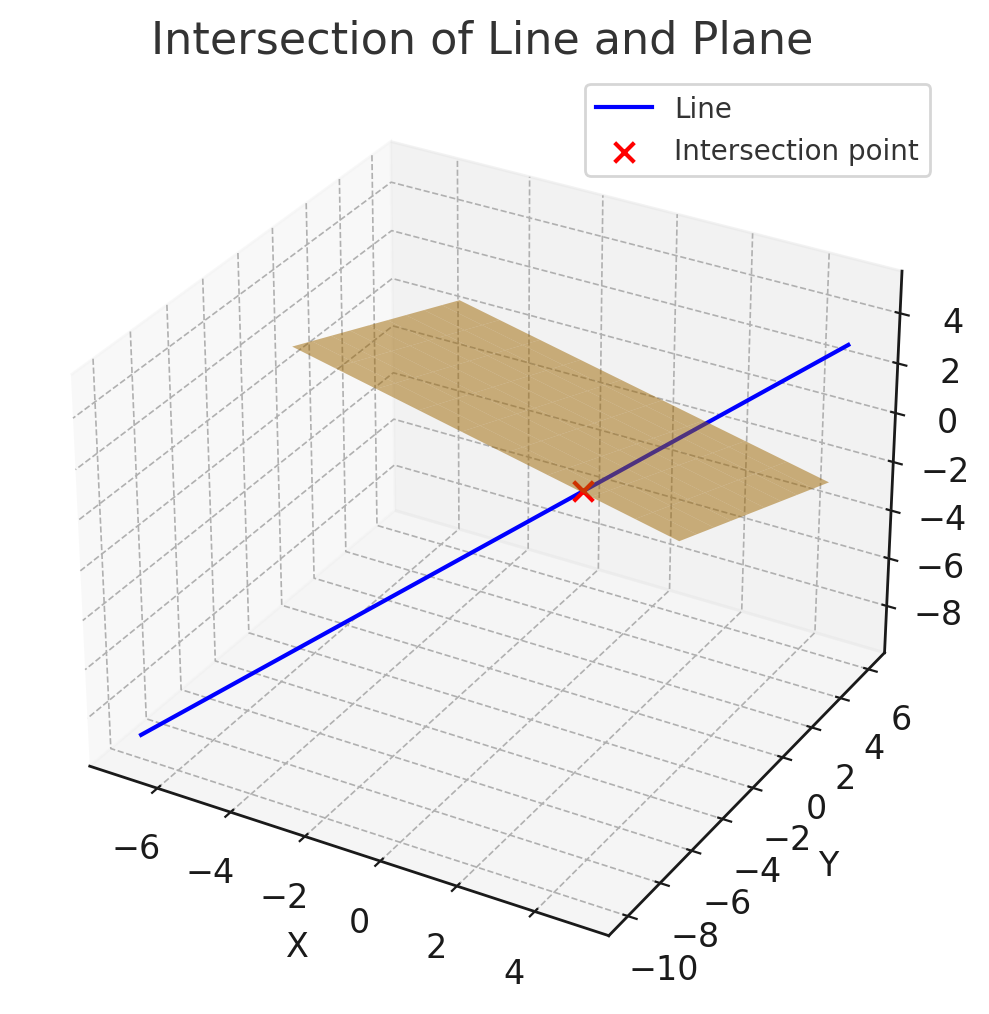
\includegraphics[width=0.8\linewidth]{figs/fig1.jpg}
    \caption{Intersection of the line with the plane}
    \label{fig:fig1}
\end{figure}

\end{document}
